\documentclass[preprint,12pt,aps,pra,showkeys,amsmath,amssymb,superscriptaddress,floatfix]{revtex4-2}
\usepackage[T1]{fontenc}
\usepackage[utf8]{inputenc}
\usepackage{amsmath,amssymb,amsthm,mathtools,mathrsfs}
\usepackage{microtype,booktabs,enumitem}
\usepackage{xcolor,tikz,etoolbox}
\usepackage[skins,breakable]{tcolorbox}
\usepackage{needspace}
% Keep diagram geometry independent of REVTeX preprint body spacing.
\AtBeginEnvironment{tikzpicture}{\linespread{1}\selectfont}
\usetikzlibrary{arrows.meta,positioning,calc,fit,decorations.pathreplacing}
\usepackage{graphicx}
\usepackage{hyperref}

\definecolor{MMBlue}{RGB}{0,82,155}
\definecolor{MMOrange}{RGB}{200,80,0}
\tikzset{
 mmnode/.style={draw=MMBlue,rounded corners=2pt,fill=MMBlue!4,align=left,execute at begin node={\raggedright},text width=5cm,font=\fontsize{10}{12}\selectfont,inner sep=6pt},
 mmimport/.style={mmnode,draw=black!65,fill=black!4},
 mmcandidate/.style={mmnode,draw=MMOrange,dashed,fill=MMOrange!5},
 mmrejected/.style={mmnode,draw=black,densely dotted,fill=black!8},
 mmproof/.style={->,thick,MMBlue},
 mmflow/.style={->,semithick,black!70},
 mmrepair/.style={->,dashed,thick,MMOrange},
 mmcandidatearrow/.style={->,dashed,semithick,MMOrange},
 mmnote/.style={font=\scriptsize,fill=white,inner sep=2pt,align=center}}

\usepackage[section]{placeins}
\setlength{\emergencystretch}{3em}
\setlist{itemsep=3pt,topsep=4pt}
\newtheorem{theorem}{Theorem}[section]
\newtheorem{proposition}[theorem]{Proposition}
\newtheorem{lemma}[theorem]{Lemma}
\newtheorem{corollary}[theorem]{Corollary}
\theoremstyle{definition}
\newtheorem{definition}[theorem]{Definition}
\newtheorem{example}[theorem]{Example}
\theoremstyle{remark}
\newtheorem{remark}[theorem]{Remark}
% Avoid isolated statement headings and single-line paragraph fragments.
\BeforeBeginEnvironment{theorem}{\Needspace{6\baselineskip}}
\BeforeBeginEnvironment{definition}{\Needspace{5\baselineskip}}
\BeforeBeginEnvironment{proposition}{\Needspace{5\baselineskip}}
\BeforeBeginEnvironment{lemma}{\Needspace{5\baselineskip}}
\BeforeBeginEnvironment{corollary}{\Needspace{5\baselineskip}}
\clubpenalty=5000
\widowpenalty=5000
\newcommand{\R}{\mathbb R}\newcommand{\Z}{\mathbb Z}\newcommand{\N}{\mathbb N}
\newcommand{\Pa}{\operatorname{Pa}}\newcommand{\Desc}{\operatorname{Desc}}
\newcommand{\cl}{\operatorname{cl}}\newcommand{\cost}{\operatorname{cost}}
\newcommand{\status}{\operatorname{status}}
% Faculty cards: a visual rail groups the five faculties within one agent.
% The rail has no arrowhead and does not represent a proof dependency.
\newcommand{\mmfacultybadge}[1]{%
 \node[circle,draw=MMBlue,line width=1pt,fill=white,
 minimum size=7mm,inner sep=0pt,font=\sffamily\small\bfseries,text=MMBlue]
 at ([xshift=15pt,yshift=-15pt]frame.north west) {#1};}
\newcommand{\mmfacultyrail}{%
 \draw[MMBlue!80,line width=1pt]
 ([xshift=15pt,yshift=2pt]frame.north west)--
 ([xshift=15pt,yshift=-2pt]frame.south west);}
\newtcolorbox{mmfacultybox}[2]{enhanced,breakable,
 colback=MMBlue!4,colframe=MMBlue!4,boxrule=0pt,arc=3pt,
 left=39pt,right=9pt,top=4pt,bottom=4pt,
 before skip=2pt,after skip=2pt,
 fontupper=\small\linespread{1.1}\selectfont,
 overlay unbroken={\mmfacultyrail\mmfacultybadge{#1}},
 overlay first={\mmfacultyrail\mmfacultybadge{#1}},
 overlay middle={\mmfacultyrail},overlay last={\mmfacultyrail}}
\newcommand{\mmfaculty}[3]{%
 \begin{mmfacultybox}{#1}{#2}
 {\sffamily\bfseries\color{MMBlue}#2}\par\smallskip #3
 \end{mmfacultybox}}
\newcommand{\agent}[9]{%
 \Needspace{8\baselineskip}
 \subsubsection{#1}
 \noindent\textbf{Object.} #2\par
 \noindent\textbf{Role.} #3\par\smallskip
 \mmfaculty{E}{Ego}{#4}
 \mmfaculty{M}{Memory}{#5}
 \mmfaculty{I}{Intellect}{#6}
 \mmfaculty{S}{Sense}{#7}
 \mmfaculty{A}{Action}{#8}
 \smallskip\noindent #9\par}

\usepackage{longtable,array,calc}
\providecommand{\tightlist}{\setlength{\itemsep}{2pt}\setlength{\parskip}{0pt}}
\makeatletter
\def\frontmatter@abstract@produce{\par\addvspace{\frontmatter@preabstractspace}%
\begingroup\prep@absbox\unvbox\absbox\post@absbox\endgroup
\addvspace{\frontmatter@postabstractspace}}
\makeatother
\newcommand{\field}[2]{\par\smallskip\noindent\textbf{#1.} #2\par}
\setlength{\emergencystretch}{5em}
\AtBeginEnvironment{verbatim}{\small\linespread{1.0}\selectfont}


\hypersetup{colorlinks=true,linkcolor=MMBlue,urlcolor=MMBlue,pdfauthor={Dibakar Sigdel}}

\begin{document}

\title{Spectral Theorem for Real Symmetric Matrices\\[4pt]\large An End-to-End Meta-Math Walkthrough}

\author{Dibakar Sigdel}

\affiliation{Mindverse Computing LLC, Lynnwood, WA 98087, USA}

\date{October 2026}

\begin{abstract}

A complete authored walkthrough of spectral theorem for real symmetric
matrices, with explicit mathematical contracts, local verification
gates, and reusable exports. The report presents the target theorem,
declared imports, a dependency graph, five-faculty node contracts, a
continuous proof, a worked example, and a hypothesis-repair audit. It is
an authored mathematical exposition, not a deployed-agent transcript or
a formal proof-assistant certificate.

\end{abstract}\maketitle\linespread{1.12}\selectfont

\noindent\textbf{LA-03 / Linear Algebra / Report v1}

\section{Target and import contract}

\begin{theorem}

For every real symmetric \(n\times n\) matrix A, there are a real
orthogonal matrix Q and a real diagonal matrix Lambda such that
\(A=Q\Lambda Q^T\).

Equivalently, Euclidean space has an orthonormal basis of eigenvectors
of A. The output includes real eigenvalues, orthogonal eigendirections,
and a reconstruction certificate. It does not claim uniqueness of an
eigenbasis within a repeated eigenspace.

\end{theorem}

\subsection{Foundations and permitted imports}

A is symmetric when \(A^{T}=A\); Q is orthogonal when \(Q^{T}Q=I\).
Import compactness of the finite-dimensional unit sphere, the extreme
value theorem, elementary differentiation, and induction on dimension.
No diagonalization theorem is imported.

\clearpage\section{Node interaction workflow}

\begin{center}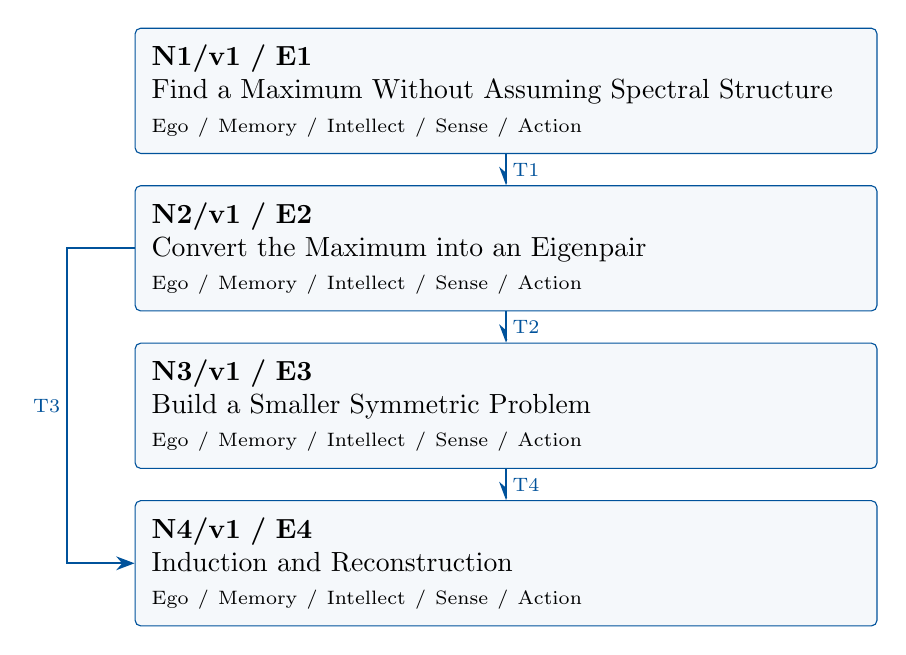
\begin{tikzpicture}[>=Stealth,x=1cm,y=1cm]

\node[mmnode,text width=9cm,minimum height=1.25cm] (N1) at (0,0.0) {\textbf{N1/v1 / E1}\\Find a Maximum Without Assuming Spectral Structure\\{\scriptsize Ego / Memory / Intellect / Sense / Action}};

\node[mmnode,text width=9cm,minimum height=1.25cm] (N2) at (0,-2.0) {\textbf{N2/v1 / E2}\\Convert the Maximum into an Eigenpair\\{\scriptsize Ego / Memory / Intellect / Sense / Action}};

\node[mmnode,text width=9cm,minimum height=1.25cm] (N3) at (0,-4.0) {\textbf{N3/v1 / E3}\\Build a Smaller Symmetric Problem\\{\scriptsize Ego / Memory / Intellect / Sense / Action}};

\node[mmnode,text width=9cm,minimum height=1.25cm] (N4) at (0,-6.0) {\textbf{N4/v1 / E4}\\Induction and Reconstruction\\{\scriptsize Ego / Memory / Intellect / Sense / Action}};

\draw[mmproof] (N1.south) -- node[mmnote,right] {T1} (N2.north);

\draw[mmproof] (N2.south) -- node[mmnote,right] {T2} (N3.north);

\draw[mmproof] (N2.west) -- (-5.58,-2) -- node[mmnote,left] {T3} (-5.58,-6) -- (N4.west);

\draw[mmproof] (N3.south) -- node[mmnote,right] {T4} (N4.north);

\end{tikzpicture}\end{center}

Each box is one mathematical agent containing all five faculties. Blue
arrows carry the versioned exports listed below. The layout gives a
reading order; only drawn arrows assert dependencies. Diagnostic repair
is separate from the proof DAG.

\clearpage\subsection{Versioned evidence-transfer ledger}

\begingroup\small\linespread{1.05}\selectfont

\Needspace{5\baselineskip}\field{T1: N1/E1/v1 to N2}{The Rayleigh quotient attains a real maximum at a unit vector \(v\).}

\field{Receiving activity}{N2: Convert the Maximum into an Eigenpair}

\field{Compatibility}{Use the same mathematical objects and hypotheses as the source export.
Receiving contract: N1/E1 and differentiable tangent curves on the
sphere.}

\Needspace{5\baselineskip}\field{T2: N2/E2/v1 to N3}{\(Av=\lambda v\) with \(\lambda=v^TAv\in\mathbb R\).}

\field{Receiving activity}{N3: Build a Smaller Symmetric Problem}

\field{Compatibility}{Use the same mathematical objects and hypotheses as the source export.
Receiving contract: N2/E2 and symmetry of the original operator.}

\Needspace{5\baselineskip}\field{T3: N2/E2/v1 to N4}{\(Av=\lambda v\) with \(\lambda=v^TAv\in\mathbb R\).}

\field{Receiving activity}{N4: Induction and Reconstruction}

\field{Compatibility}{Use the same mathematical objects and hypotheses as the source export.
Receiving contract: N2/E2, N3/E3, and induction on dimension.}

\Needspace{5\baselineskip}\field{T4: N3/E3/v1 to N4}{\(v^\perp\) is invariant under \(A\), and the restriction there is
symmetric of dimension \(n-1\).}

\field{Receiving activity}{N4: Induction and Reconstruction}

\field{Compatibility}{Use the same mathematical objects and hypotheses as the source export.
Receiving contract: N2/E2, N3/E3, and induction on dimension.}

\endgroup

\clearpage\section{Agent roles and five-faculty activities}\begingroup\small\linespread{1.05}\selectfont\setlist{itemsep=1pt,topsep=2pt}

\subsection{N1/v1: Find a Maximum Without Assuming Spectral Structure}

\field{Object and role}{Find a Maximum Without Assuming Spectral Structure. Establish the
following local result: The Rayleigh quotient attains a real maximum at
a unit vector \(v\).}

\field{Inputs}{A real symmetric \(n\times n\) matrix, \(n\ge1\); compactness of the
unit sphere.}

\mmfaculty{E}{Ego}{Own E1/v1: The Rayleigh quotient attains a real maximum at a unit vector
\(v\).}

\mmfaculty{M}{Memory}{Symmetry and Euclidean inner product}

\mmfaculty{I}{Intellect}{Study quadratic form on unit sphere}

\mmfaculty{S}{Sense}{Require finite dimension and real symmetry}

\mmfaculty{A}{Action}{Carry out the numbered deductions and publish E1/v1 together with its
hypotheses and proof location.}

\smallskip\noindent\textbf{Numbered mathematical activities}

\begin{enumerate}[label=N1.\arabic*,leftmargin=3.4em]

\item Restrict \(x^TAx\) to the unit sphere.

\item Check continuity and apply the extreme value theorem.

\item Fix a maximizing unit vector without assuming any spectral
decomposition.

\end{enumerate}

\field{Export E1/v1}{The Rayleigh quotient attains a real maximum at a unit vector \(v\).}

\field{Acceptance gate}{Require finite dimension and real symmetry Publish only after checking
every displayed deduction.}

\field{Targeted repair}{If the check fails, revise N1: Require finite dimension and real
symmetry Recheck dependent nodes N2, N3, N4.}

\clearpage

\subsection{N2/v1: Convert the Maximum into an Eigenpair}

\field{Object and role}{Convert the Maximum into an Eigenpair. Establish the following local
result: \(Av=\lambda v\) with \(\lambda=v^TAv\in\mathbb R\).}

\field{Inputs}{N1/E1 and differentiable tangent curves on the sphere.}

\mmfaculty{E}{Ego}{Own E2/v1: \(Av=\lambda v\) with \(\lambda=v^TAv\in\mathbb R\).}

\mmfaculty{M}{Memory}{Maximum and tangent curves}

\mmfaculty{I}{Intellect}{Differentiate at maximizing point}

\mmfaculty{S}{Sense}{Avoid assuming eigenvector existence}

\mmfaculty{A}{Action}{Carry out the numbered deductions and publish E2/v1 together with its
hypotheses and proof location.}

\smallskip\noindent\textbf{Numbered mathematical activities}

\begin{enumerate}[label=N2.\arabic*,leftmargin=3.4em]

\item For each \(w\perp v\), differentiate along
\((v+tw)/\sqrt{1+t^2\|w\|^2}\).

\item The derivative vanishes at the maximum, giving \(w^TAv=0\).

\item Therefore \(Av\) lies in the line spanned by \(v\).

\end{enumerate}

\field{Export E2/v1}{\(Av=\lambda v\) with \(\lambda=v^TAv\in\mathbb R\).}

\field{Acceptance gate}{Avoid assuming eigenvector existence Publish only after checking every
displayed deduction.}

\field{Targeted repair}{If the check fails, revise N2: Avoid assuming eigenvector existence
Recheck dependent nodes N3, N4.}

\clearpage

\subsection{N3/v1: Build a Smaller Symmetric Problem}

\field{Object and role}{Build a Smaller Symmetric Problem. Establish the following local result:
\(v^\perp\) is invariant under \(A\), and the restriction there is
symmetric of dimension \(n-1\).}

\field{Inputs}{N2/E2 and symmetry of the original operator.}

\mmfaculty{E}{Ego}{Own E3/v1: \(v^\perp\) is invariant under \(A\), and the restriction
there is symmetric of dimension \(n-1\).}

\mmfaculty{M}{Memory}{Symmetric inner-product identity}

\mmfaculty{I}{Intellect}{Reduce dimension orthogonally}

\mmfaculty{S}{Sense}{Restriction must remain invariant and symmetric}

\mmfaculty{A}{Action}{Carry out the numbered deductions and publish E3/v1 together with its
hypotheses and proof location.}

\smallskip\noindent\textbf{Numbered mathematical activities}

\begin{enumerate}[label=N3.\arabic*,leftmargin=3.4em]

\item For \(w\perp v\), compute \(\langle Aw,v\rangle=\langle w,Av\rangle=0\).

\item Restrict the symmetric inner-product identity to the invariant subspace.

\item Prepare the smaller-dimensional induction problem.

\end{enumerate}

\field{Export E3/v1}{\(v^\perp\) is invariant under \(A\), and the restriction there is
symmetric of dimension \(n-1\).}

\field{Acceptance gate}{Restriction must remain invariant and symmetric Publish only after
checking every displayed deduction.}

\field{Targeted repair}{If the check fails, revise N3: Restriction must remain invariant and
symmetric Recheck dependent nodes N4.}

\clearpage

\subsection{N4/v1: Induction and Reconstruction}

\field{Object and role}{Induction and Reconstruction. Establish the following local result:
\(A=Q\Lambda Q^T\) for an orthogonal \(Q\) and real diagonal
\(\Lambda\).}

\field{Inputs}{N2/E2, N3/E3, and induction on dimension.}

\mmfaculty{E}{Ego}{Own E4/v1: \(A=Q\Lambda Q^T\) for an orthogonal \(Q\) and real diagonal
\(\Lambda\).}

\mmfaculty{M}{Memory}{Lower-dimensional result}

\mmfaculty{I}{Intellect}{Combine orthonormal bases}

\mmfaculty{S}{Sense}{Handle repeated eigenvalues}

\mmfaculty{A}{Action}{Carry out the numbered deductions and publish E4/v1 together with its
hypotheses and proof location.}

\smallskip\noindent\textbf{Numbered mathematical activities}

\begin{enumerate}[label=N4.\arabic*,leftmargin=3.4em]

\item Apply the theorem inductively on \(v^\perp\), starting with dimension
one.

\item Join its orthonormal eigenbasis with \(v\).

\item Check \(Q^TAQ=\Lambda\) and the reconstruction
\(A=\sum_i\lambda_i v_iv_i^T\).

\end{enumerate}

\field{Export E4/v1}{\(A=Q\Lambda Q^T\) for an orthogonal \(Q\) and real diagonal
\(\Lambda\).}

\field{Acceptance gate}{Handle repeated eigenvalues Publish only after checking every displayed
deduction.}

\field{Targeted repair}{If the check fails, revise N4: Handle repeated eigenvalues Withhold this
terminal result until its gate passes.}

\endgroup\clearpage\section{Continuous mathematical proof}\label{sec:proof}

\subsection{N1 --- Find a Maximum Without Assuming Spectral
Structure}\label{n1-find-a-maximum-without-assuming-spectral-structure}

For \(n\ge 1\), the function \(R(x)=x^TAx\) is continuous on the compact
unit sphere. It attains a maximum at a unit vector v. Set
\(\lambda =v^{T}Av\), which is real. This constructs a candidate
eigenvector through optimization rather than assuming one exists.

\subsection{N2 --- Convert the Maximum into an
Eigenpair}\label{n2-convert-the-maximum-into-an-eigenpair}

Let w be any vector perpendicular to v, and consider

\[x(t)=\frac{v+tw}{\sqrt{1+t^2\|w\|^2}}.\]

This stays on the unit sphere, \(x(0)=v\), and x'\((0)=w\). Since
\(R(x(t))\) has a maximum at zero, its derivative there vanishes.
Symmetry gives

\[0=\left.\frac d{dt}x(t)^TAx(t)\right|_{t=0}=w^TAv+v^TAw=2w^TAv.\]

Thus Av is orthogonal to every vector in v-perp, so Av is a multiple of
v. Taking its inner product with v gives \(Av=\lambda v\). This
establishes a real eigenpair for every nonzero-dimensional symmetric
operator.

\subsection{N3 --- Build a Smaller Symmetric
Problem}\label{n3-build-a-smaller-symmetric-problem}

For u in v-perp,

\[v^TAu=(Av)^Tu=\lambda v^Tu=0.\]

Hence Au remains in v-perp: this subspace is invariant. The restricted
operator is symmetric because
\(\langle Au,w\rangle=\langle u,Aw\rangle\) still holds for u,w there.

The restriction acts on an \((n-1)\)-dimensional Euclidean space. The
proof has now generated a smaller instance of the same theorem, with the
hypotheses preserved.

\subsection{N4 --- Induction and
Reconstruction}\label{n4-induction-and-reconstruction}

For \(n=1\) the theorem is immediate. Assume it in dimension \(n-1\).
Apply it to the N3 restriction to obtain an orthonormal eigenbasis of
v-perp. Adjoin v to get an orthonormal eigenbasis \(v_1,\ldots,v_n\) of
the original space.

Let Q have those vectors as columns and let Lambda contain their
eigenvalues. Then \(AQ=Q\) Lambda and \(Q^{T}Q=I\). Thus
\(Q^TAQ=\Lambda\) and \(A=Q\Lambda Q^T\). This closes the induction.
\(\square\)

As a further consequence,

\[A=\sum_{j=1}^n\lambda_jv_jv_j^T.\]

Different eigenvalues have perpendicular eigenvectors: if \(Au=\lambda\)
u and \(Av=mu\) v, symmetry gives \((\lambda-\mu)u^Tv=0\). Repeated
eigenvalues are handled by an orthonormal basis within their eigenspace;
they do not obstruct the theorem.

\hfill$\square$

\section{Worked orchestration}

Take

\[A=\begin{pmatrix}2&1&0\\1&2&0\\0&0&4\end{pmatrix}.\]

The quadratic form is \(2x^2+2xy+2y^2+4z^2\). Since \(2xy\le x^2+y^2\),
it is at most \(3(x^2+y^2)+4z^2\le4\) on the unit sphere, with equality
at \(e_{3}\). N2 therefore supplies eigenpair \((4,e_{3})\).

N3 restricts to the xy-plane. Its matrix is {[}{[}2,1{]},{[}1,2{]}{]},
with orthonormal eigenvectors

\[v_1=\frac1{\sqrt2}(1,1,0),\quad\lambda_1=3;\qquad v_2=\frac1{\sqrt2}(1,-1,0),\quad\lambda_2=1.\]

Together with \(v_{3}=e_{3}\) and lambda \(_{3}=4\), take

\[Q=\begin{pmatrix}1/\sqrt2&1/\sqrt2&0\\1/\sqrt2&-1/\sqrt2&0\\0&0&1\end{pmatrix},\qquad\Lambda=\operatorname{diag}(3,1,4).\]

Action verifies \(Q^{T}Q=I\), \(Av_j=\lambda _j\) \(v_j\), and the
reconstruction. The first two spectral contributions are

\[3v_1v_1^T+v_2v_2^T=\begin{pmatrix}2&1&0\\1&2&0\\0&0&0\end{pmatrix},\]

while \(4v_3v_3^T\) supplies the last diagonal entry.

\subsection{Boundary and hypothesis audit}

Symmetry is essential: {[}{[}1,1{]},{[}0,1{]}{]} has only one
independent eigenvector and cannot be diagonalized. A real rotation may
have no real eigenvalues. Positive eigenvalues are not required:
symmetric matrices can have negative eigenvalues. The zero matrix is
covered and permits any orthonormal basis.

Export the extremal-eigenvector lemma, invariant-complement lemma,
orthogonal diagonalization, and rank-one spectral reconstruction. These
are the exact imports used to develop singular value decomposition in
the problem bank.

\section{Illustrative failure and repair}

The following is an authored diagnostic scenario. Changed assumptions
define a new contract; they do not retroactively prove the original
statement.

\subsection{Failure and correction}
Suppose a branch normalizes several independently chosen eigenvectors
and assumes they are orthogonal. For \(A=I\), \(e_{1}\) and
\(e_{1}+e_{2}\) are both eigenvectors, but normalization alone does not
make them orthogonal.

\begin{itemize}
\item
  \textbf{Node:} N4
\item
  \textbf{State:} STALLED
\item
  \textbf{Failing faculty:} Action
\item
  \textbf{Failed claim:} normalized eigenvectors form orthogonal Q
\item
  \textbf{Observed:} off-diagonal entry of Q transpose Q is nonzero
\item
  \textbf{Repair target:} basis selection
\item
  \textbf{Blocked export:} orthogonal diagonalization certificate
\end{itemize}

Memory recalls orthogonal complements and repeated eigenspaces. Sense
checks whether the chosen vectors are independent. Intellect constructs
an orthonormal basis in the repeated eigenspace. Action verifies its
inner products and that every new vector remains an eigenvector. Ego
republishes the decomposition only after \(Q^{T}Q=I\) holds.

\subsection{Hypothesis boundary}
Symmetry is essential: {[}{[}1,1{]},{[}0,1{]}{]} has only one
independent eigenvector and cannot be diagonalized. A real rotation may
have no real eigenvalues. Positive eigenvalues are not required:
symmetric matrices can have negative eigenvalues. The zero matrix is
covered and permits any orthonormal basis.

Export the extremal-eigenvector lemma, invariant-complement lemma,
orthogonal diagonalization, and rank-one spectral reconstruction. These
are the exact imports used to develop singular value decomposition in
the problem bank.

\subsection{Version and recheck}
Treat any changed assumption as a new contract. Recheck the revised
export and all of its descendants. A backward diagnostic never
establishes an earlier theorem. This is an authored teaching trace, not
an execution log.

\par\medskip\begingroup\small\linespread{1.0}\selectfont\noindent\textbf{Provenance.} This authored proof is complete relative to its declared imports. Reuse
each export with its assumptions, proof, and version. The original
Markdown remains available for comparison.
\par\endgroup

\par\smallskip\begingroup\small\linespread{1.0}\selectfont\noindent\textbf{Further reading.} \href{https://ocw.mit.edu/courses/18-700-linear-algebra-fall-2013/pages/study-materials/}{MIT
linear algebra: proof of the spectral theorem}.\par\endgroup

\end{document}
